
%----------------------------------------
\begin{frame}
  \frametitle{Placing numbers in a sequence of trays}\small
  \centering
  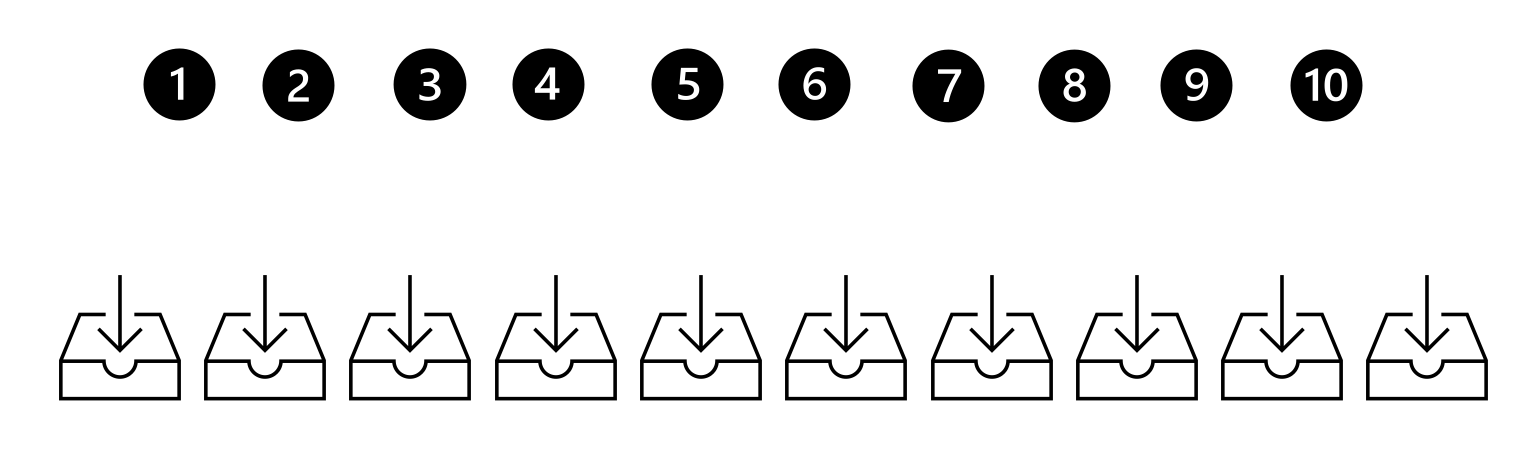
\includegraphics[width=\textwidth]{figures/balls.png}

  \begin{block}{}\scriptsize
    \begin{itemize}
    \item After 2 should eventually follow 6.   
    \item After 7 all numbers should be bigger than 7.
    \item A 1 should be preceded in the past by  a 3.
  \end{itemize}
\end{block}

\end{frame}

%----------------------------------------
\begin{frame}
  \vspace{1.2cm}

  \frametitle{Placing numbers in a sequence of trays}\small
  \centering
  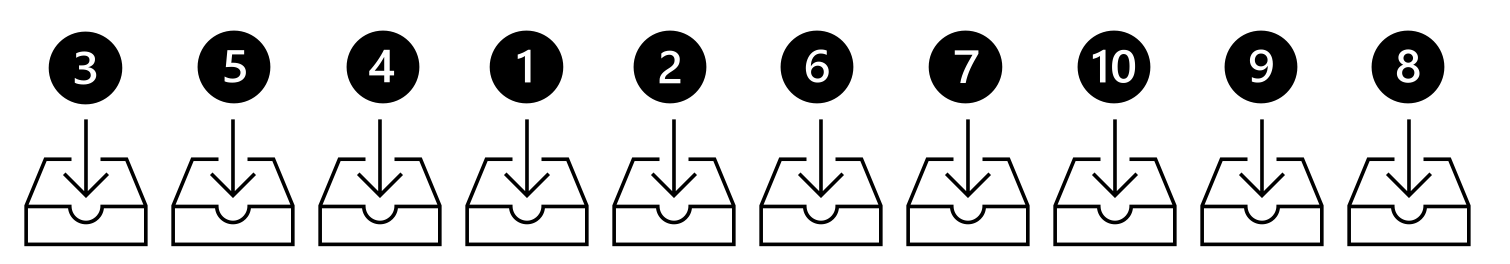
\includegraphics[width=\textwidth]{figures/balls-assigned.png}

  \vspace{0.3cm}

  \begin{block}{}\scriptsize
    \begin{itemize}
    \item After 2 should eventually follow 6.   
    \item After 7 all numbers should be bigger than 7.
    \item A 1 should be preceded in the past by  a 3.
  \end{itemize}
\end{block}
  
\end{frame}

%----------------------------------------
\begin{frame}[fragile]
  \frametitle{Modeling temporal logic in first-order logic on a finite trace} \small

\begin{block}{Consider the first temporal property}\scriptsize
\begin{itemize}
\item After 2 should eventually follow 6. 
\end{itemize}

\[
\Box (2 \rightarrow \Diamond 6)
\]

\begin{lstlisting}[language=tasknetdsl,frame=single]
                        always (2 implies eventually 6);
\end{lstlisting}

\end{block}

\pause

\vspace{0.2cm}
{\bf It can be translated to a first-order logic formula constraining $tray$:}

\[
\forall i \in \{1..k\},\ tray(i) = 2 
  \rightarrow 
    \exists j \in \{i..k\}, tray(j) = 6
\]

\pause

\vspace{0.2cm}
{\bf Then we can ask an SMT solver such as Z3\\ 
\url{https://github.com/Z3Prover/z3}\\ 
to find an assignment of numbers to trays positions that satisfies this formula.}

\end{frame}